
%% bare_conf.tex
%% V1.4b
%% 2015/08/26
%% by Michael Shell
%% See:
%% http://www.michaelshell.org/
%% for current contact information.
%%
%% This is a skeleton file demonstrating the use of IEEEtran.cls
%% (requires IEEEtran.cls version 1.8b or later) with an IEEE
%% conference paper.
%%
%% Support sites:
%% http://www.michaelshell.org/tex/ieeetran/
%% http://www.ctan.org/pkg/ieeetran
%% and
%% http://www.ieee.org/

%%*************************************************************************
%% Legal Notice:
%% This code is offered as-is without any warranty either expressed or
%% implied; without even the implied warranty of MERCHANTABILITY or
%% FITNESS FOR A PARTICULAR PURPOSE! 
%% User assumes all risk.
%% In no event shall the IEEE or any contributor to this code be liable for
%% any damages or losses, including, but not limited to, incidental,
%% consequential, or any other damages, resulting from the use or misuse
%% of any information contained here.
%%
%% All comments are the opinions of their respective authors and are not
%% necessarily endorsed by the IEEE.
%%
%% This work is distributed under the LaTeX Project Public License (LPPL)
%% ( http://www.latex-project.org/ ) version 1.3, and may be freely used,
%% distributed and modified. A copy of the LPPL, version 1.3, is included
%% in the base LaTeX documentation of all distributions of LaTeX released
%% 2003/12/01 or later.
%% Retain all contribution notices and credits.
%% ** Modified files should be clearly indicated as such, including  **
%% ** renaming them and changing author support contact information. **
%%*************************************************************************


% *** Authors should verify (and, if needed, correct) their LaTeX system  ***
% *** with the testflow diagnostic prior to trusting their LaTeX platform ***
% *** with production work. The IEEE's font choices and paper sizes can   ***
% *** trigger bugs that do not appear when using other class files.       ***                          ***
% The testflow support page is at:
% http://www.michaelshell.org/tex/testflow/



\documentclass[conference]{IEEEtran}
% Some Computer Society conferences also require the compsoc mode option,
% but others use the standard conference format.
%
% If IEEEtran.cls has not been installed into the LaTeX system files,
% manually specify the path to it like:
% \documentclass[conference]{../sty/IEEEtran}


% *** CITATION PACKAGES ***
%
\usepackage{cite}
% cite.sty was written by Donald Arseneau
% V1.6 and later of IEEEtran pre-defines the format of the cite.sty package
% \cite{} output to follow that of the IEEE. Loading the cite package will
% result in citation numbers being automatically sorted and properly
% "compressed/ranged". e.g., [1], [9], [2], [7], [5], [6] without using
% cite.sty will become [1], [2], [5]--[7], [9] using cite.sty. cite.sty's
% \cite will automatically add leading space, if needed. Use cite.sty's
% noadjust option (cite.sty V3.8 and later) if you want to turn this off
% such as if a citation ever needs to be enclosed in parenthesis.
% cite.sty is already installed on most LaTeX systems. Be sure and use
% version 5.0 (2009-03-20) and later if using hyperref.sty.
% The latest version can be obtained at:
% http://www.ctan.org/pkg/cite
% The documentation is contained in the cite.sty file itself.



% *** GRAPHICS RELATED PACKAGES ***
%

\usepackage{graphicx}
\graphicspath{{fig/}}


% *** MATH PACKAGES ***
%
\usepackage{amsmath}
\interdisplaylinepenalty=2500


% *** ALIGNMENT PACKAGES ***
%
\usepackage{array}

% *** SUBFIGURE PACKAGES ***
\ifCLASSOPTIONcompsoc
 \usepackage[caption=false,font=normalsize,labelfont=sf,textfont=sf]{subfig}
\else
  \usepackage[caption=false,font=footnotesize]{subfig}
\fi

\hyphenation{optical networks semi-conductor}
\usepackage{tikz}
\usetikzlibrary{arrows}

\tikzset{
    left/.style={circle, draw=blue, fill=blue},
    dele/.style={circle, draw=black, fill=black},
    decision/.style={circle, draw=red, fill=red}
}
\begin{document}
%
% paper title
% Titles are generally capitalized except for words such as a, an, and, as,
% at, but, by, for, in, nor, of, on, or, the, to and up, which are usually
% not capitalized unless they are the first or last word of the title.
% Linebreaks \\ can be used within to get better formatting as desired.
% Do not put math or special symbols in the title.
\title{Joint Equalization and Decoding Scheme\\ using Modified Spinal Codes\\ for Underwater Communications}


% author names and affiliations
% use a multiple column layout for up to three different
% affiliations
\author{\IEEEauthorblockN{Yupeng TAI}
\IEEEauthorblockA{State Key Laboratory\\ Acoustics
Institute of Acoustics,\\
Chinese Academy of Sciences \\
Beijing, China}
\and
\IEEEauthorblockN{Frederic GUILLOUD, Christophe LAOT\\ and Raphael LE BIDAN}
\IEEEauthorblockA{SC department\\ 
Telecom Bretagne Institut Mines-Telecom\\ 
Brest, France}
\and
\IEEEauthorblockN{Haibin WANG}
\IEEEauthorblockA{State Key Laboratory\\ Acoustics
Institute of Acoustics,\\
Chinese Academy of Sciences \\
Beijing, China}}

% conference papers do not typically use \thanks and this command
% is locked out in conference mode. If really needed, such as for
% the acknowledgment of grants, issue a \IEEEoverridecommandlockouts
% after \documentclass

% for over three affiliations, or if they all won't fit within the width
% of the page, use this alternative format:
% 
%\author{\IEEEauthorblockN{Michael Shell\IEEEauthorrefmark{1},
%Homer Simpson\IEEEauthorrefmark{2},
%James Kirk\IEEEauthorrefmark{3}, 
%Montgomery Scott\IEEEauthorrefmark{3} and
%Eldon Tyrell\IEEEauthorrefmark{4}}
%\IEEEauthorblockA{\IEEEauthorrefmark{1}School of Electrical and Computer Engineering\\
%Georgia Institute of Technology,
%Atlanta, Georgia 30332--0250\\ Email: see http://www.michaelshell.org/contact.html}
%\IEEEauthorblockA{\IEEEauthorrefmark{2}Twentieth Century Fox, Springfield, USA\\
%Email: homer@thesimpsons.com}
%\IEEEauthorblockA{\IEEEauthorrefmark{3}Starfleet Academy, San Francisco, California 96678-2391\\
%Telephone: (800) 555--1212, Fax: (888) 555--1212}
%\IEEEauthorblockA{\IEEEauthorrefmark{4}Tyrell Inc., 123 Replicant Street, Los Angeles, California 90210--4321}}




% use for special paper notices
%\IEEEspecialpapernotice{(Invited Paper)}




% make the title area
\maketitle

% As a general rule, do not put math, special symbols or citations
% in the abstract
\begin{abstract}
To get the optimal intersymbol interference(ISI) cancelling performance over the highly frequency-selective underwater acoustic channel(UAC), the classical iterating joint equalization and decoding should have to use large interleaver size to  lower the correlation between the soft informations which the equalizer pass on the decoder. However, it brings in additional deteriorations when the interleaver block is longer than the channel coherence  time of UAC. Therefore, it rise great interesting to seek for a scheme that could cancelling the major ISI with a short coding block. This paper provide a novel attempt to solve this problem by proposing a non-iterating joint equalization and decoding scheme using the modified spinal code. The linear-complexity approximate maximum likelihood(ML) estimation is used in the scheme. It's efficient even over the large delay spread channels.  For most channels with different level of frequency-selectivity, the proposed scheme provides competitive  performance, especially for high spectral efficiency modulations. A simulation with UAC extract form actual sea experiments is present at the end of this paper which shows the  excellent performances consistent with the universal frequency-selective channel simulations.
\end{abstract}

% no keywords




% For peer review papers, you can put extra information on the cover
% page as needed:
% \ifCLASSOPTIONpeerreview
% \begin{center} \bfseries EDICS Category: 3-BBND \end{center}
% \fi
%
% For peerreview papers, this IEEEtran command inserts a page break and
% creates the second title. It will be ignored for other modes.
\IEEEpeerreviewmaketitle


%------------------------------------------------------------------------------------------
\section{Introduction}
% no \IEEEPARstart
The underwater acoustic channel(UAC) is known as a time-varying intersymbol interference(ISI) channel. In the area of underwater acoustic communication, ISI cancelling is always an active topic. A turbo equalizer\cite{douillard1995iterative}
allows the receiver to benefit from the channel decoder gain by using a iterative process joint the equalizer and decoder. The equalizer produce the estimates of transmitted symbols using different methods. The maximum likelihood (ML) estimation is the optimal method in getting the minimum bit error rate (BER). However, the complexity of such methods often remains significantly high, especially for channels with large delay spread like the UAC. So some linear optimization algorithms are selected such as zero forcing (ZF) or minimum mean squared error (MMSE) estimation.   
Results shows that the linear MMSE(LE-MMSE) turbo equalizer could completely remove the ISI for a time-invariant and averagely frequency-selective channel with acceptable complexity \cite{laot2001turbo}. However, it's hard for the LE-MMSE  turbo equalizer to achieve a satisfied performance for the highly frequency-selective channel unless the interleaver block  is very long. However, it also makes the interleaving block longer than the coherence  time of UAC which deteriorates the performance on another side. This is a practical contradiction in using the LE-MMSE Turbo equalization for UAC.


In this paper, a novel joint equalization and decoding scheme based on a modified fixed-rate spinal code is proposed. It is aimed to provide a acceptable performance for a large range of channels using a smaller code block length.  

Spinal code is newly designed \cite{perry2012spinal}
random number generator based channel coding method. Its core idea is sequentially apply the hash function to generate a set of original seed numbers which is used to seed a pseudo-random mapping function to produce a sequence of symbols for transmission. 

There is two aspects of the spinal code which is quite different with the previous channel codes. First, it uses the invertible hash function which makes it impossible to  implement the graphical or algebraic decoding method as previous codes. So the decoding method of spinal code is an tree structure algorithm with the approximate maximum likelihood (ML)estimation method. As the powerful mixing effect of hash function, the approximate ML decoder is quite efficient. This is also the foundation that makes the proposed approximate joint equalization and decoding method could achieve a satisfactory performance within linear time complexity even for the channel with large delay spread.  
Another difference is that it encode the bits directly to constellation symbols and decoding the bits with the hard information directly extract from the symbols. Benefit from this point and the sequential structure of decoder,it's easy to add the equalization into the process of decoding without using an iteration scheme and avoid the loss during the conversion from the symbols to soft information.  
%------------------------------------------------------------------------------------------
\section{The Transmission Scheme}
The transmission scheme is diagrammed by Fig.\ref{fig_tranScheme}, the core hash function part $H$ is fed by independent binary message date $m_k$ and produce a set of $v$-bits seeds $s_k$. After puncturing the remained set $\widehat{s}_k$ is took by the random mapper to generated the output symbols $x_n$ to the ISI channel. 

The signal is deteriorate by the ISI channel and the AWGN noise $w_n$ with variance $\sigma^2_w$. The received channel output could represented by:
\begin{equation}
y_n=\sum_{l=0}^Lh_lx_{n-l}+w_n 
\label{equ_yn}
\end{equation}
where $h_l$ are the coefficients of the discrete channel impulse response with the length of $L$. 

The definition of signal-to-noise SNR in this paper is:
\begin{equation}
SNR=\frac{E_s}{N_0}
\label{equ_snr}
\end{equation}
where $E_s$ is the mean energy of $y_n$. $N_0$ is the monolateral power spectral density of $w_n$.
% to be continue
% You must have at least 2 lines in the paragraph with the drop letter
% (should never be an issue)	
\begin{figure}[!t]
\centering
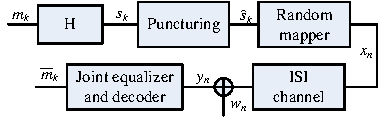
\includegraphics[width=3.0 in]{tranScheme.pdf}
\caption{The transmission scheme}
\label{fig_tranScheme}
\end{figure}
%------------------------------------------------------------------------------------------
\section{The Modified Spinal Code}
We implement a new kind of fixed-rate spinal code which is less complexity and more suitable for the combination with equalization.
%------------------------------------------------------------------------------------------
\subsection{Encoding Method}
%------------------------------------------------------------------------------------------
\subsubsection{Pseudo-Random Hash Function}
The core of the spinal code is a recursive structure constructed by a pseudo-random hash function, . As shown in Fig. \ref{fig_hash}, the $H$ takes two inputs: a $v$-bits seed $s_{i-1}$ and one bit of message $m_i$ and returns a $v$-bits seed $s_i$ which is also the next input seed. Additionally, the initial seed value, $s_0$ is a constant value which is known to both the sender and the receiver.
\begin{figure}[!t]
\centering
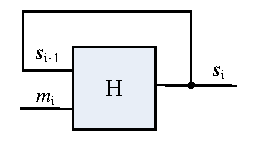
\includegraphics[width=2 in]{encoderCore.pdf}
\caption{The core hash structure}
\label{fig_hash}
\end{figure}
%------------------------------------------------------------------------------------------
\subsubsection{The Random Mapper}

The set of $k$ seeds ($k$ is the length of the message) is used to seed a random mapper. There is a range of candidate  mapper method for the random mapper: it could be a combination of  a random number generator(RNG) and a usual mapper (constellation mapper for QAM or subcarrier mapper for OFDM, etc.) %or directly use the random mapper methods.

Our implementation is consisted with a random number generator and a constellation mapper as shown in Fig. \ref{fig_mapper} where C-mapper represent the constellation mapper and the $x_{i,1},x_{i,2},...,x_{i,q}$ is the output sub-block of $q$-symbols  under the seed of  $s_i$. Given that the bit per symbol number of mapper output is $c$, then the code rate $R=k/cqk=1/cq$
\begin{figure}[!t]
\centering
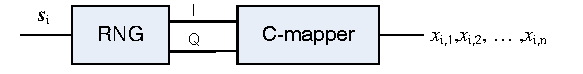
\includegraphics[width=3 in]{mapper.pdf}
\caption{The random mapper}
\label{fig_mapper}
\end{figure}
%------------------------------------------------------------------------------------------
\subsubsection{Puncturing}
As the $q$ is a integer bigger than 1. So the maximum code rate of previous encoding structure is $1/c$ which is quite low when the SNR is high. 

Puncturing maybe a good choice to conquer this problem. Instead of sending all the seeds into the mapper, the sender skips some of the seeds with a preset puncturing pattern. Given the puncture rate is $p$, the code rate after puncturing turns into $R=p/cq$.
Benefit from the strongly sequential structure of the encode method. The spinal code could support high puncturing rate. This provide a larger adjusting range for the spinal code.

In our implement the puncturing method is kind of strided puncturing with the consistent strided distance $p$ whose puncturing pattern is $P=[b_1,b_2,...,b_p]$ where only $b_1=1$ and the rests are set to 0. 
\begin{figure}[!t]
\centering
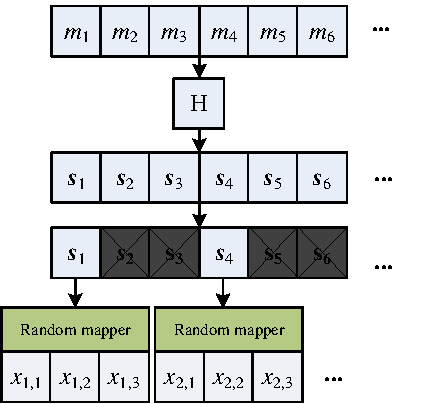
\includegraphics[width=3 in]{punturing.pdf}
\caption{The puncturing structure}
\label{fig_puncturing}
\end{figure}
%------------------------------------------------------------------------------------------
\subsection{Approximate ML Decoder}
The basic concept of the optimal ML decoder is 	redo the encoder with all the potential message bit sequences. And find the one with minimum distance from the received symbol set. So the ML rule for the AWGN channel is:
\begin{equation}
\widehat{\textbf{m}}=\underset{\textbf{m}\in\{0,1\}^k}{\arg\min}\Vert\textbf{y}-\textbf{x}(\textbf{m})\Vert^2
\label{equ_ml}
\end{equation}
where $\textbf{y}$ is the received vector and $\textbf{x}(\textbf{m})$ is the transmitted symbols yield by encoder with message vector \textbf{m}.
As the  symbols produced by the random-mappers seeded by the same $s_i$ would be coincident with each other, \textbf{y} could be decomposed into $\textbf{y}_1,\textbf{y}_2,...,\textbf{y}_{k/p}$ sub-victors who shares the same seeds. Disregard the puncturing, the cost function would be:
\begin{equation}
\Vert\textbf{y}-\textbf{x}(\textbf{m})\Vert^2=\sum_{i=1}^{k}\Vert\textbf{y}_{i}-\textbf{x}_{i}(s_{i})\Vert^2
\label{equ_cost0}
\end{equation}
Given the addition of $p$-rate strided puncturing and $t =(i-1)p+1$ which is index of the seed who generated $x_i$, the cost function changed into:
\begin{equation}
\sum_{i=1}^{\frac{k}{p}}\Vert\textbf{y}_{i}-\textbf{x}_{i}(s_{t})\Vert^2
\label{equ_cost1}
\end{equation}
Further break the sub-vectors $\textbf{y}_i$ into $y_{(i-1)q+1},y_{(i-1)q+2},...,y_{qi}$, we could get the final  cost function:%add explaination
\begin{equation}
\sum_{i=1}^{\frac{k}{p}}\sum_{j=q(i-1)+1}^{qi}\vert y_{j}-x_{j}(s_{t})\vert^2
\label{equ_cost2}
\end{equation}
Based on (\ref{equ_cost2}) the sequential structure of the encoder. The ML decode of spinal code could be recast as a searching for the minimum distant path over a binary tree. The tree is rooted from $s_0$, each node has two edge $e_{m_i}(s_i,s_{i+1})$ connect to two children represent the two possible choices of input bit $m_i$. The total depth of the tree is $k$. So $2^k$ path should be take into count to construct such a binary tree for the optimal ML decoder. This is too complex. 

Fortunately, benefit from the hash function and random generators used, the simply classical approximate ML algorithm which is termed \textit{M-algorithm} in \cite{Anderson1984} shows near optimal performance within linear complexity. The main idea of this algorithm is only maintain $B$ subtrees and prune the rest within each depth increase on the tree. 

Fig. \ref{fig_decoderTree} shows an example of decoder tree with $B$ equal to 2 where the blue node represent the remained, the black nodes represent the pruned and the path consist by red nodes is the final decision of the decoder.%new added

The \textit{M-algorithm} is simple but very efficient in decoding spinal code. That owe to the pairwise independence properties of hash function and random generators. That is, any pair of messages who have the same first $i$ bits and only different from the bits with index higher than $i$ will generated sets of symbols who have the same $iq$ symbols(ignore the puncturing). While their remained subsets are entirely independent of each other.
\begin{figure}
\centering
\begin{tikzpicture}
  [
    grow                    = right,
    sibling distance        = 3cm,
    level distance          = 2cm,
    every node/.style       = {font=\footnotesize},
  ]
  \node [decision] {}
    child { [sibling distance=1.2cm] node [decision] {}
    	child { [sibling distance=1.2cm] node [dele] {}}
    	child { [sibling distance=1.2cm]node [decision] {}
    	    child{node[dele] {}}
    		child{node[decision] {}
    		    child{node[decision]{}}
    			child{node[left]{}}}}}
    child {[sibling distance=1.2cm] node [left] {}
        child {[sibling distance=1.2cm] node [left] {}
            child{node[dele] {}}
    		child{node[left] {}
    			child{node[left]{}}
    			child{node[left]{}}}}
    	child { [sibling distance=1.2cm]node [dele] {}}}
    ;
\end{tikzpicture}
\caption{Tree structure of decoder}
\label{fig_decoderTree}
\end{figure}
%------------------------------------------------------------------------------------------
\section{Proposed Joint Decoding and Equalization Scheme}
%--------------------------------------------------------------------------------------------
\subsection{The Approximate ML joint Decoding and Equalization}
Consider cost function (\ref{equ_cost2}) under ISI channel expressed by (\ref{equ_yn}), we got the cost function under ISI channel:
\begin{equation}
\sum_{i=1}^{\frac{k}{p}}\sum_{j=q(i-1)+1}^{qi}\vert y_{j}-\sum_{l=1}^L x_{j-l}(s_{t})\vert^2
\label{equ_costEqu}
\end{equation}
where $t=\lfloor\frac{j-l}{q}\rfloor p+1$

Base on (\ref{equ_costEqu}) and apply the approximate ML method \textit{M-algorithm} again. We got the tree structure of approximate ML joint equalization and decoding scheme.


%--------------------------------------------------------------------------------------------
\subsection{Time Complexity}
The decoding process requires $k$ steps of expanding on the tree. Each step expand $2B$ node with costs of a hush computation. Among the steps, $k/p$ steps involve in $q$ random number generation, and $Lq$ multiplication for replay the channel convolution. The selection for the best $B$ of each step candidates need $O(2B)$ operation with proper algorithm. 

\begin{table}[!t]
\renewcommand{\arraystretch}{1.3}
\centering
\caption{Number of required operations per symbol of proposed scheme}
\label{tab_ComplexitySpinal}
\begin{tabular}{|c||c|}
\hline
operation &amount \\
\hline
hash\&RNG  & $2B(p+q)/q$\\
\hline
multiplications& $2BL$\\
\hline
comparison & $O(2Bp/q)$\\
\hline

\end{tabular}

\end{table}

So we got the number of required operations per symbol of proposed scheme showed in table \ref{tab_ComplexitySpinal}. We can see that if $B$ is constant, the complexity is linear in $k$. And it has no relationship with bit per symbol number $c$. That means we could freely use high-degree modulation without worrying about additional complexity. 

In comparison,  Turbo equalization requires several iterations between the BCJR \cite{1055186} decoder and LE-MMSE equalization or MAP equalization. The BCJR algorithm for convolution decoder requires $O(2^{\overline{M}}k)$ operations where $\overline{M}$ is the memory length of the code. The LE-MMSE equalization need $O((N^2+L^2)k)$ operations,where $N$ is the filter length. The MAP equalization need $O(2^{cL}k)$ operations. 
%\begin{table}[!hbp]
%\label{tab_ComplexityCompare}
%\centering
%\caption{comparison in number of required operation} 
%\begin{tabular}{|c|c|}
%\hline
%approach & operations\\
%\hline
%proposed scheme & $O(2Bk)$\\
%
%turbo equalization(MAP)& $O((2^{\overline{M}}+2^{cL})k)$\\
%
%turbo equalization(LE-MMSE)& $O((2^{\overline{M}}+N^2+L^2)k)$\\
%\hline
%
%\end{tabular}
%
%\end{table}
With a proper selection of parameters, the proposed scheme requires a comparable number of operations per symbols to the LS-MMSE Turbo equalization and much more efficient than the MAP Turbo equalization especially when the channel delay is large. The proposed scheme have some additional advantages in efficiency, such it's parallelizable and it could run during the symbol receiving.
%--------------------------------------------------------------------------------------------
\section{Simulation Results}
%--------------------------------------------------------------------------------------------
\subsection{Universal Frequency-selective Channel}
For easily comparing the results with other schemes, the constellation mapper used in random mapper is $M$-QAM mapper. The universal frequency-selective channels used in this section are proposed by Proakis \cite{proakis}:
\begin{equation}
\begin{split}
H_{Proakis A}=&[0.04, -0.05, 0.07, -0.21, -0.5,\\ &0.72, 0.36, 0, 0.21, 0.03, 0.07]^T\\
H_{Proakis B}=&[0.417, 0.815, 0.407]^T\\
H_{Proakis C}=&[0.227, 0.460, 0.688, 0.460, 0.227]^T\\
\end{split}
\end{equation}
\begin{figure}[!t]
\centering
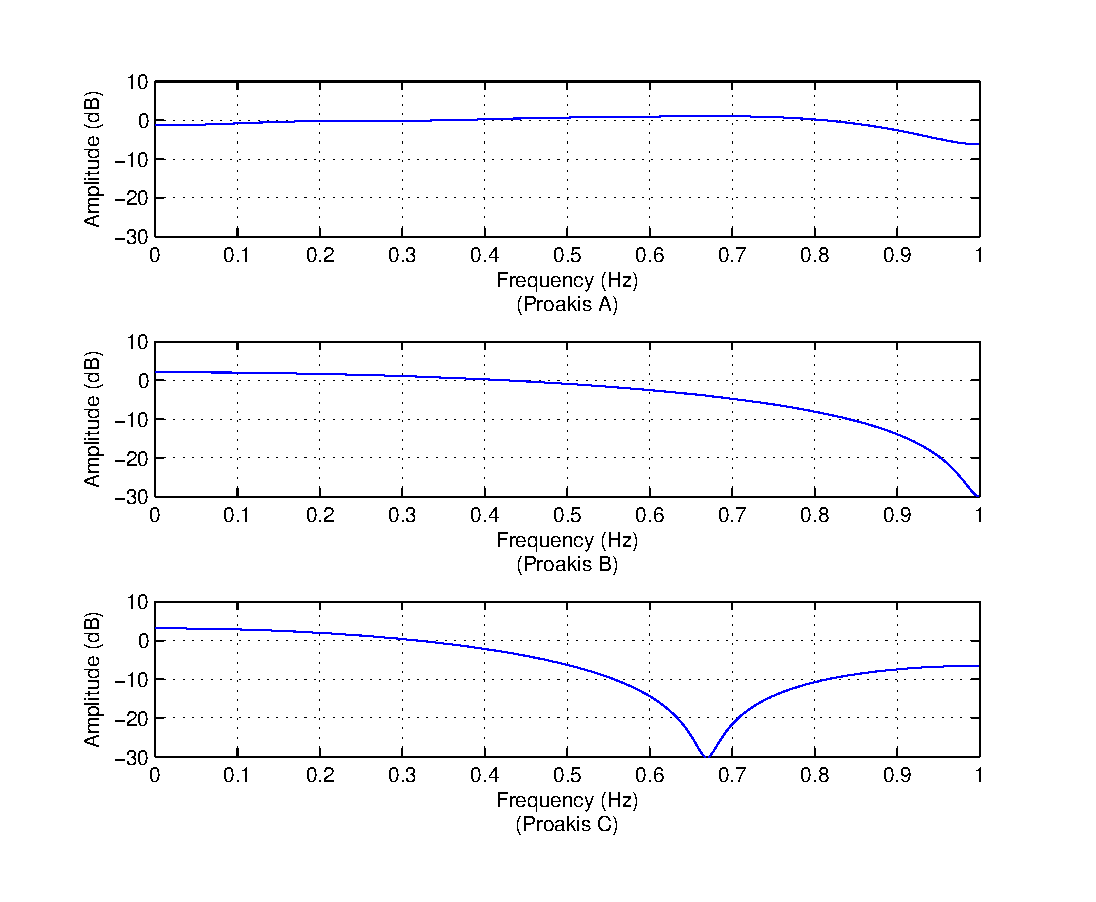
\includegraphics[width=3 in]{PorakisBCchannelResponse.eps}
\caption{The amplitude-frequency responses}
\label{fig_channel}
\end{figure}
whose amplitude-frequency response is showed in Fig. \ref{fig_channel}.

We found that the modified 1/2-rate spinal code with parameters: $k=96, B=1024, q=2, p=2$ has the comparability both in the complexity and the BER performance with the 1/2-rate convolution code whose memory length equal to 6 and generator polynomials equal to 163,135 (expressed in octals) with QPSK signaling scheme over AWGN channel. So they are selected respectively to apply into the proposed scheme and Turbo equalization for comparing there performance over frequency-selective channel.  
\begin{figure}[!t]
\centering
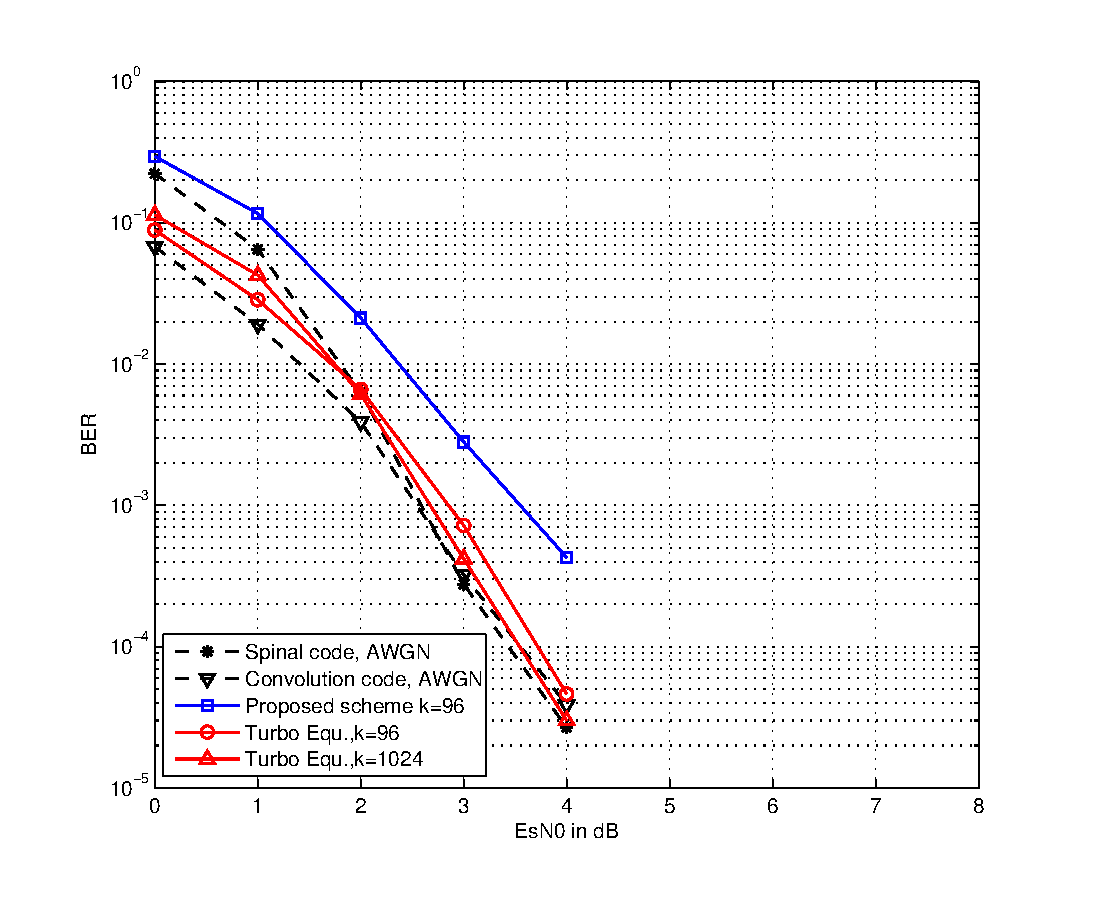
\includegraphics[width=3 in]{ChAQPSKComparison.eps}
\caption{The performance of proposed scheme and Turbo equalization over Porakis A channel for QPSK modulation}
\label{fig_ChAQPSKComparison}
\end{figure}

\begin{figure}[!t]
\centering
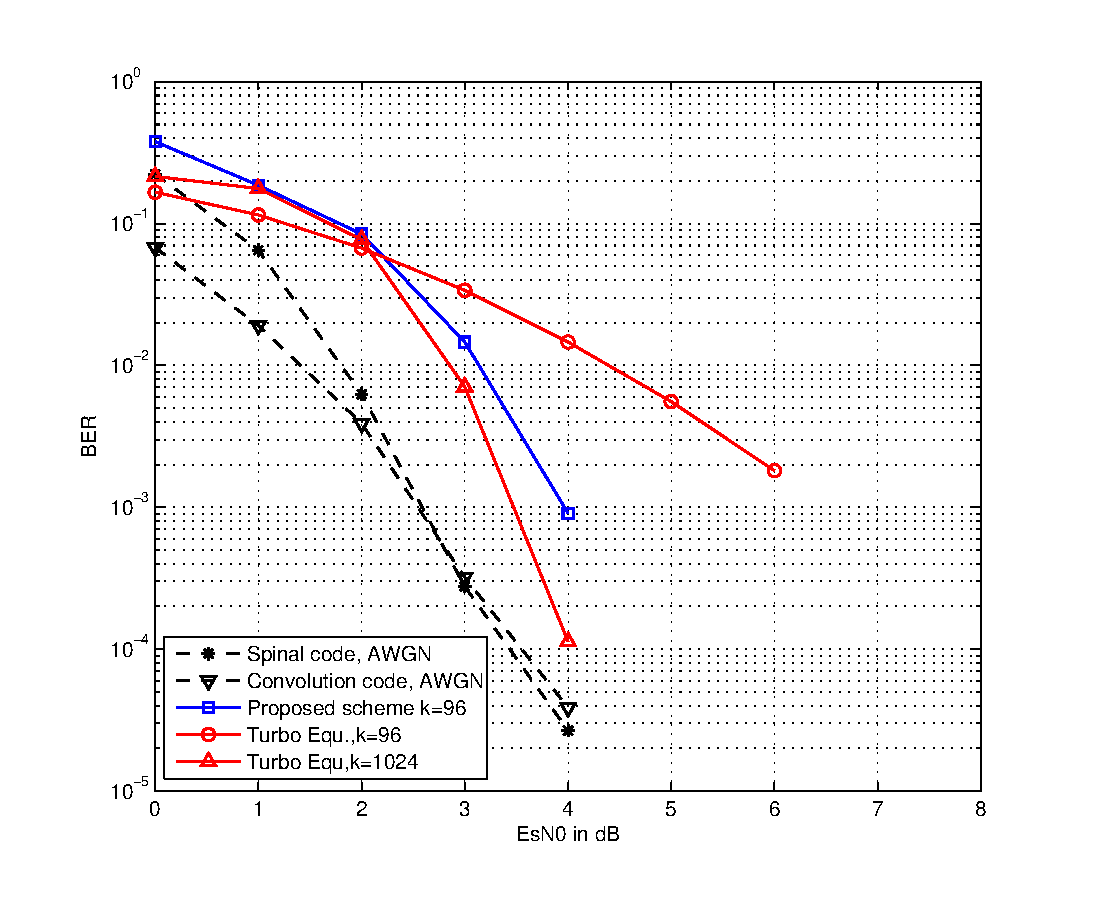
\includegraphics[width=3 in]{ChBQPSKComparison.eps}
\caption{The performance of proposed scheme and Turbo equalization over Porakis B channel for QPSK modulation}
\label{fig_ChBQPSKComparison}
\end{figure}

\begin{figure}[!t]
\centering
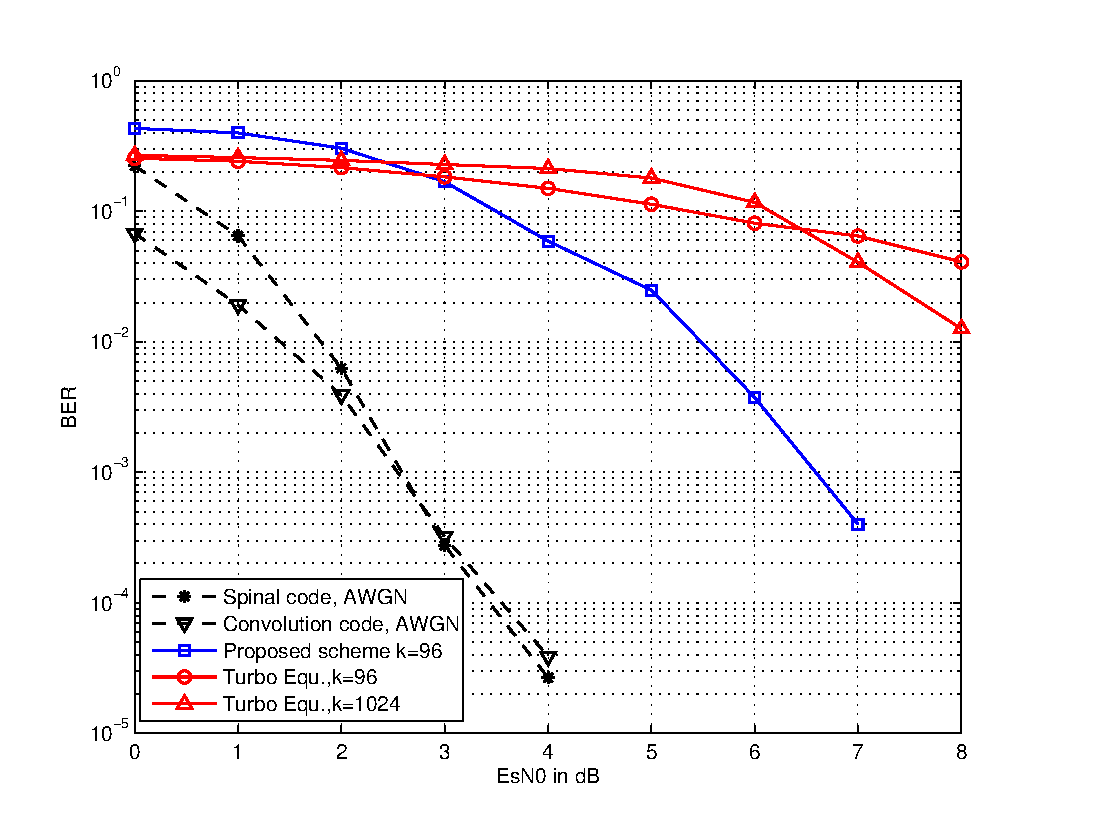
\includegraphics[width=3.1 in]{ChCQPSKComparison.eps}
\caption{The performance of proposed scheme and Turbo equalization over Porakis C channel for QPSK modulation}
\label{fig_ChCQPSKComparison}
\end{figure}
Fig. \ref{fig_ChAQPSKComparison}, Fig. \ref{fig_ChBQPSKComparison} and Fig. \ref{fig_ChCQPSKComparison}  present the performance of proposed scheme and Turbo equalization at the fifth iteration over Porakis A Porakis B and Porakis C channels respectively.  The results show that the proposed scheme could get better performance when the block length is short over highly frequency-selective channels . While, it shows the bigger gap to the theoretical bound with the lower frequency-selective channel. It is because the sub-optimal ML equalization requires more time complexity to erase the final gap to the theoretical bound.
\begin{figure}[!t]
\centering
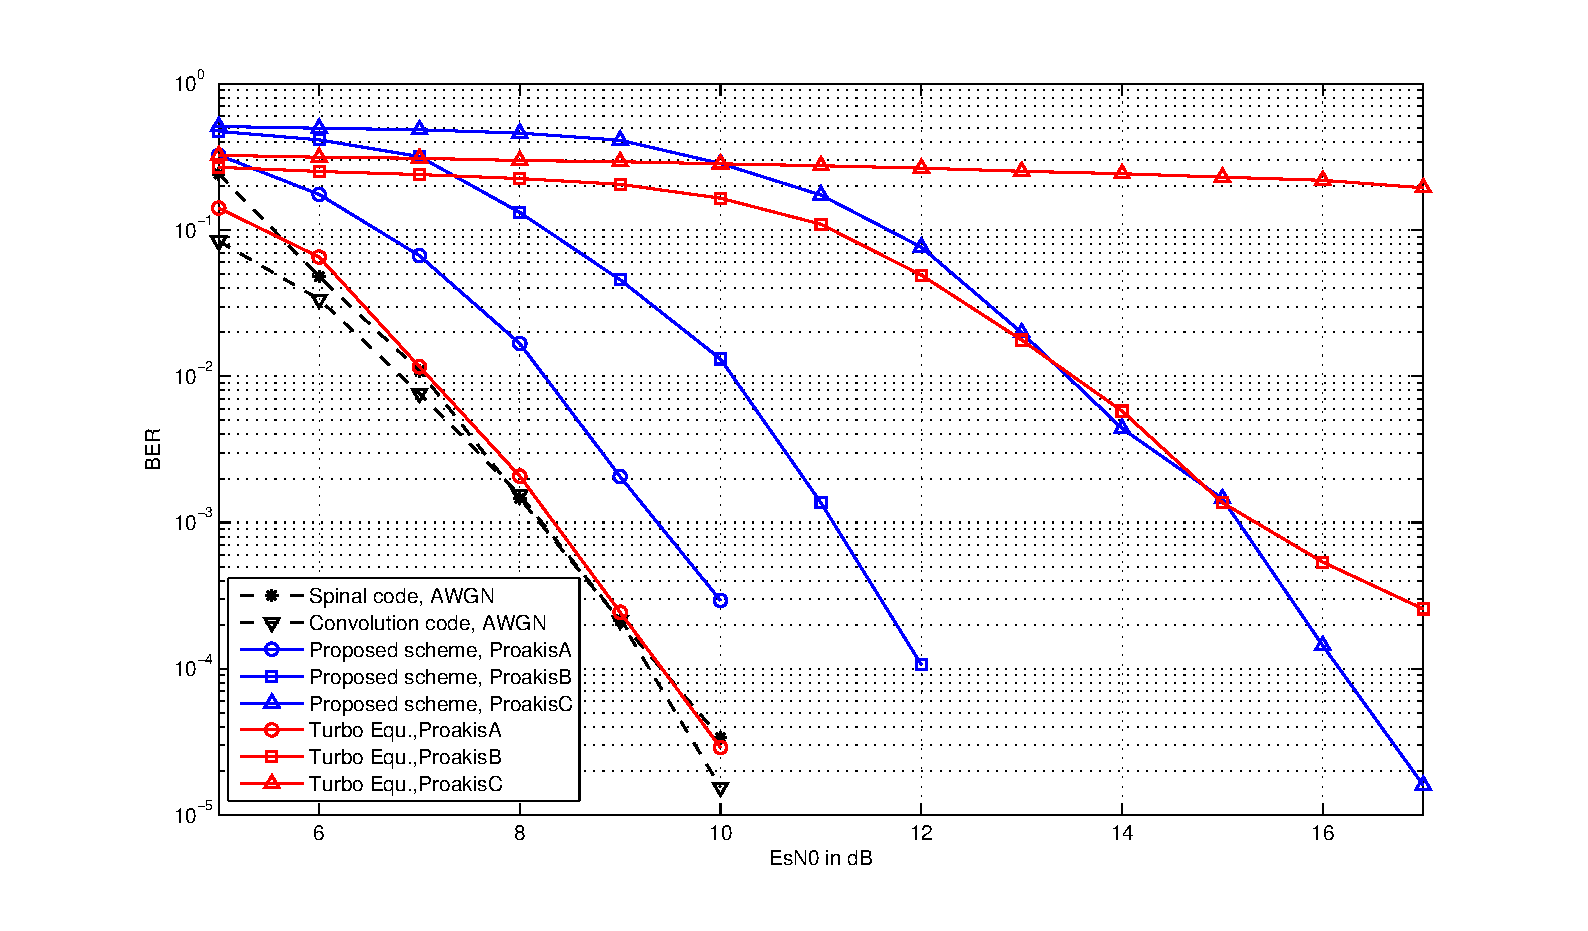
\includegraphics[width=3.5 in]{16QAMComparison.eps}
\caption{The performance of proposed scheme and Turbo equalization at the fifth iteration for 16QAM modulation}
\label{fig_16QAMComparison}
\end{figure}
Fig. \ref{fig_16QAMComparison} shows the performances of proposed scheme and Turbo equalization evaluated for 16QAM signaling scheme. To stay comparability with Turbo equalization and maintain the code rate at 1/2. The sub-block length $p$ of modified Spinal code is adjusted to 1. 

From Fig. \ref{fig_16QAMComparison} we can see the performances gap between proposed scheme and Turbo equalization over Proakis B and Proakis C channel expand in the signaling scheme of 16QAM. For these highly frequency-selective channels, it's hard for the equalizer of Turbo equalization to get a feed of estimated date with BER lower than the threshold to allowed the "turbo effect" primed. Whereas the proposed scheme isn't a iterate structure, so their is no "BER threshold" problem.%This is just my analise. Don't know if it's reasonable.

%--------------------------------------------------------------------------------------------
\subsection{Underwater Acoustic Channels Extracted from Sea Experiment}

%-------------------------------------------------------------------
\subsubsection{Shallow Sea Underwater Acoustic Channel}
This channel is estimated from the data of an underwater acoustic communication experiment carry out on the South China Sea in 2011 by Institute of Acoustic(IOA), Chinese academy of sciences (CAS). The channel coefficients and  amplitude-frequency responses are represent in Fig. \ref{fig_ShallowChannel}. The channel amplitude-frequency response is smooth except a notch at the normalized frequency 0.2. 
\begin{figure}[!t]
\centering
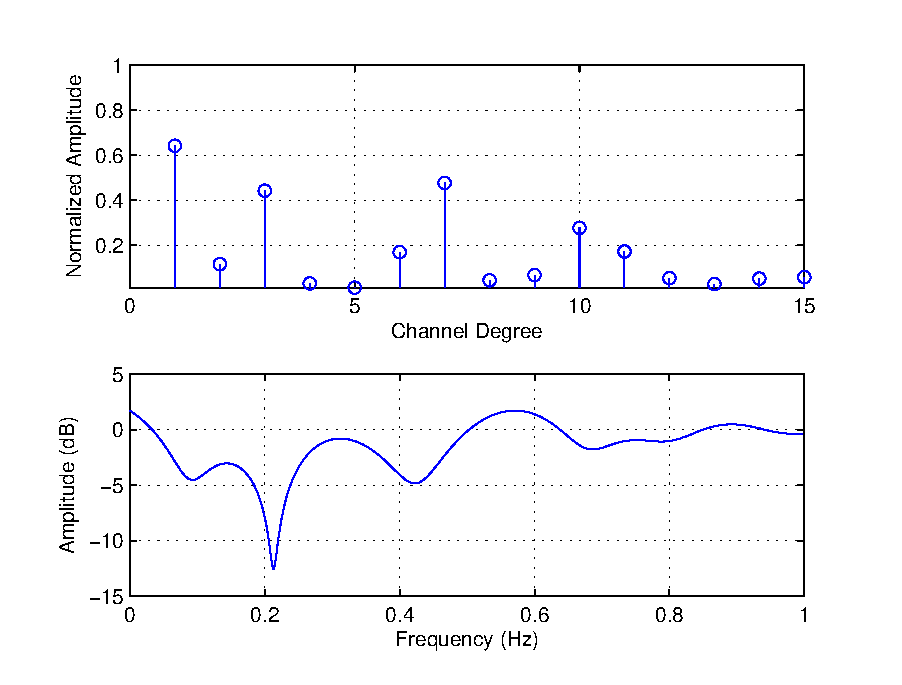
\includegraphics[width=3.5 in]{ShallowChannel.eps}
\caption{The amplitude-time and amplitude-frequency responses of a shallow-sea UAC}
\label{fig_ShallowChannel}
\end{figure}
The performance of proposed scheme and the Turbo equalization over this channel is presented in Fig. \ref{fig_ShallowQPSKComparison}. The proposed scheme also shows the stable performance with small block length.
\begin{figure}[!t]
\centering
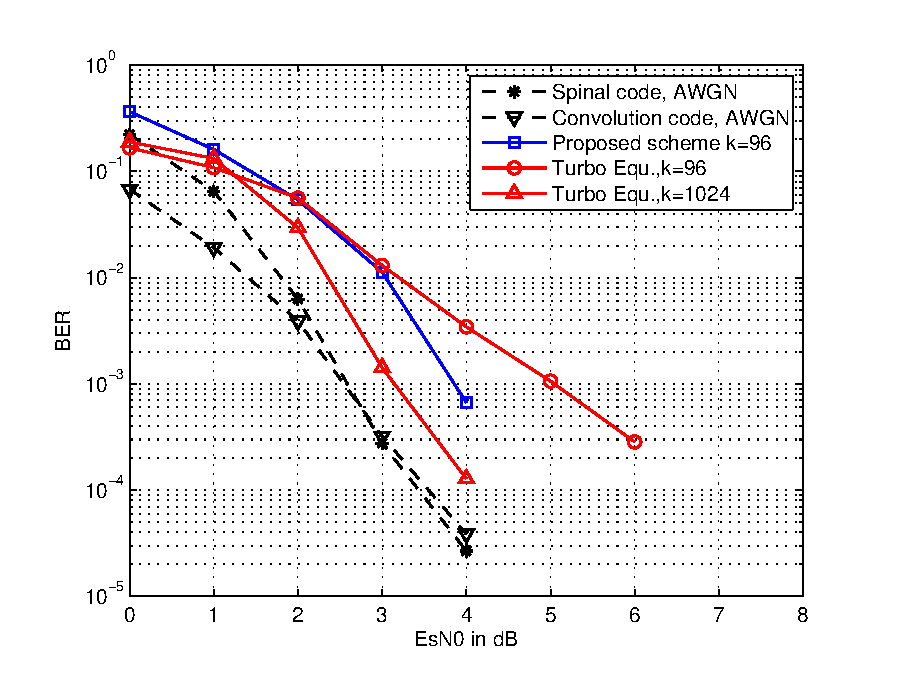
\includegraphics[width=3.5 in]{ShallowQPSKComparison.eps}
\caption{The performance of proposed scheme and Turbo equalization over shallow-sea UAC}
\label{fig_ShallowQPSKComparison}
\end{figure}
%--------------------------------------------------------------------------
\subsubsection{Deep Sea Underwater Acoustic Channel}
Fig. \ref{fig_DeepChannel} shows the deep sea channel extracted form the data of an experiment carry out in South China Sea at 2013 by IOA. The water depth of experiment area is 5000m. The distance between sender an receiver is 69km which exactly in the second  shadow zone of  the transmission loss curve. The channel is deteriorated by a strong multipath signal  with a delay if 100 symbol periods.

\begin{figure}[!t]
\centering
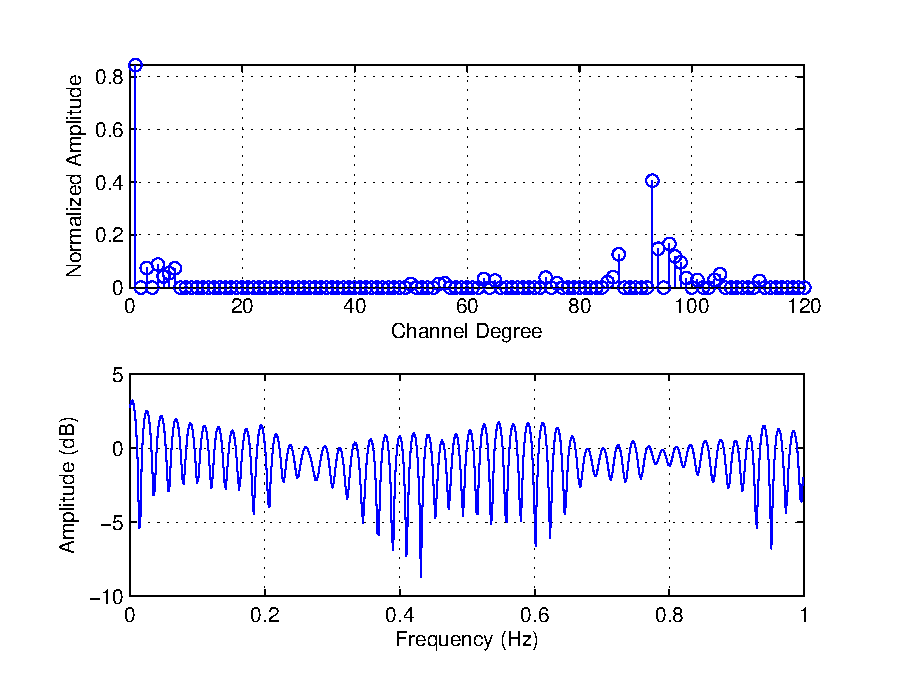
\includegraphics[width=3 in]{DeepChannel.eps}
\caption{The amplitude-time and amplitude-time responses of deep-sea underwater acoustic channel}
\label{fig_DeepChannel}
\end{figure}
The results is showed in Fig. \ref{fig_DeepQPSKComparison} 

\begin{figure}[!t]
\centering
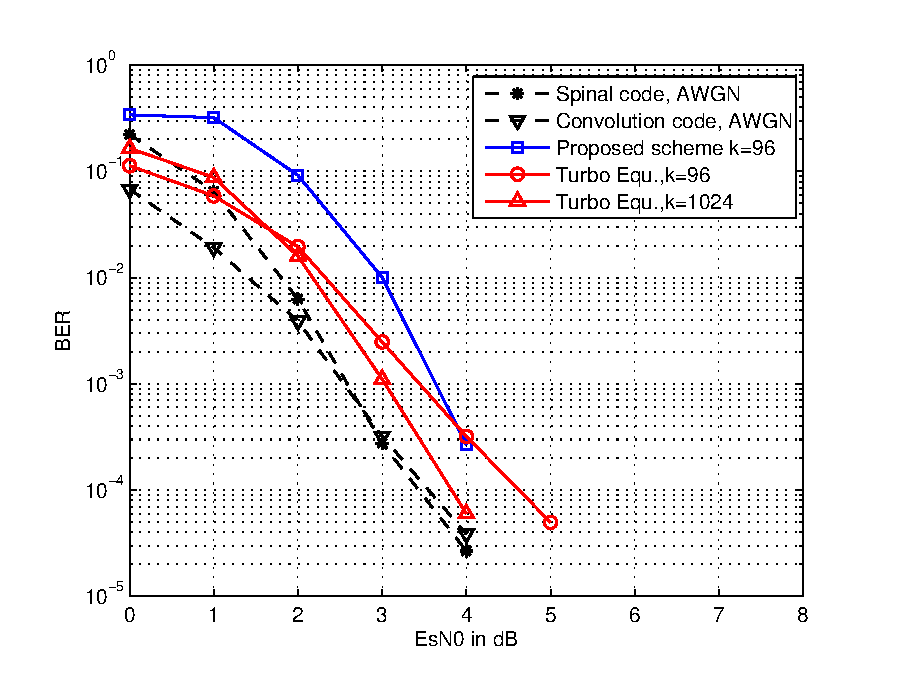
\includegraphics[width=3.5 in]{DeepQPSKComparison.eps}
\caption{The performance of proposed scheme and Turbo equalization over deep-sea UAC}
\label{fig_DeepQPSKComparison}
\end{figure}

%One thing to be mentioned, the filter length of Turbo Equalization is  set to 120 to equal with the channel length.  I'm not sure if it is the proper method to deal with the large delay channel? Would a equalization with such long filter practicable? So I don't know if we should drop this simultaion. I just want to show that complexity for such a large delay channel is still acceptable. But I found it's hard to assess it. 

\section{Conclusion}
This paper represent the design and performance analysis of modified spinal code and a joint equalization and decoding scheme using it. The approximate ML method is applied in the scheme with linear time complexity.  This non-iterative receiver scheme shows stable and acceptable performance for a larger range of channels in small code block length. The performance gap between the proposed scheme and the LE-MMSE turbo equalization is as large as 6dB over the highly frequency-selective Proakis B channel using 16QAM modulation method. 

This paper shows a newly attempt to overcome the ISI in UAC with a limited code block length. It also leaves aspect to explore for the future work. First, the approximate is not perfect enough to remove all ISI totally. The performance always leaves a small gap to the theoretical bound. Second, the addition of channel estimation and the performance analysis for time-varying channels is also interesting to explore. The last but not the least, the coding scheme is a newly designed, their is a bunch of similar structure and realizations. It's also interesting to seek the one for better overcoming the channel ISI of UAC.






\bibliographystyle{IEEEtran}
\bibliography{IEEEabrv,OceanConf_full}

\end{document}


